\chapter{Fetch Limited }

\section{Purpose}
The goal of this test-case is to validate the generation (Source/sink terms)  and the growth of the wave spectrum depending of the length of wind action (fetch) with a constant wind defined at 10 meters from the sea surface. The domain used is simple and we want to observe the evolution of few parameters along its length, as the significant wave height, peak period and variance spectrum.
It is supposed that the wind blew long enough to have reached a steady state.\\
Thus, this benchmark will allow us to compare and validate the different models of wind generation (three models), whitecapping dissipation (two models), non-linear quadruplet interactions (three models but only two are used here). Friction bottom dissipation and eventually depth-induced breaking dissipation (four models) is also included when a finite depth is imposed. The models used are presented in the Table \ref{tab:fetch_lim_models}.

\begin{table}[H]
\begin{center}
%
\footnotesize
%
\caption{Different models used for this test-case. In all cases, linear wave growth term from the formula of Cavaleri and
Malanotte-Rizzoli (1981) is used.\textit{* : Discrete Interaction Approximation,Hasselmann et al., 1985. ** : Gaussian Quadrature Method,introduced by Lavrenov
\cite{Lavrenov2001} and implemented by Benoit and Gagnaire-Renou \cite{Gagnaire2010}}}
\label{tab:fetch_lim_models}
%
\begin{tabular*}{\linewidth}{@{\extracolsep{\fill}}ccccccc}
\toprule
\toprule
\textbf{Models} & \textbf{\minitab[c]{Wind \\ generation \\ model}}
& \textbf{\minitab[c]{White \\ capping \\ model}}
& \textbf{\minitab[c]{Quadruplet \\ transfers \\ formula}} & \textbf{Depth}
& \textbf{\minitab[c]{Bottom \\ friction \\ coeff.}} &
\textbf{\minitab[c]{Depth-induced \\ breaking \\ dissipation \\ model}} \\
\midrule
test 1 & Janssen \citep{Janssen1989,Janssen1991} &
\minitab[c]{Komen \citep{Komen1984} \& \\ Janssen \citep{Janssen1991}} &
DIA* & $\inf$ & -- & -- \\
\midrule
test 2  & Snyder \citep{Snyder1981} &
\minitab[c]{Komen \citep{Komen1984} \& \\ Janssen \citep{Janssen1991}} &
DIA* & $\inf$ & -- & -- \\
\midrule
test 3  & Snyder \citep{Snyder1981} &
Westhuysen \citep{Westhuys2007} &
DIA* & $\inf$ & -- & -- \\
\midrule
test 4  & Yan \citep{Yan1987} &
Westhuysen \citep{Westhuys2007} &
DIA* & $\inf$ & -- & -- \\
\midrule
test 5  & Snyder \citep{Snyder1981} &
Westhuysen \citep{Westhuys2007} &
\minitab[c]{Exact GQM** \\ coarse \\ discretization} &
$\inf$ & -- & -- \\
\midrule
test 6  & Janssen \citep{Janssen1989,Janssen1991} &
\minitab[c]{Komen \citep{Komen1984} \& \\ Janssen \citep{Janssen1991}} &
\minitab[c]{Exact GQM** \\ coarse \\ discretization} &
$\inf$ & -- & -- \\
test 6b  & Janssen \citep{Janssen1989,Janssen1991} &
\minitab[c]{Komen \citep{Komen1984} \& \\ Janssen \citep{Janssen1991}} &
\minitab[c]{Exact GQM** \\ medium \\ discretization} &
$\inf$ & -- & -- \\
\midrule
test 7a  & Snyder \citep{Snyder1981} &
Westhuysen \citep{Westhuys2007} &
DIA* & $180$ & $0.038$ & -- \\
test 7b  & Snyder \citep{Snyder1981} &
Westhuysen \citep{Westhuys2007} &
DIA* & $60$ & $0.038$ & -- \\
test 7c  & Snyder \citep{Snyder1981} &
Westhuysen \citep{Westhuys2007} &
DIA* & $30$ & $0.038$ & -- \\
test 7d  & Snyder \citep{Snyder1981} &
Westhuysen \citep{Westhuys2007} &
DIA* & $15$ & $0.038$ & -- \\
test 7e  & Snyder \citep{Snyder1981} &
Westhuysen \citep{Westhuys2007} &
DIA* & $5$ & $0.038$ & 
\minitab[c]{Battjes \& \\ Janssen \\ (V = 20m/s)} \\
\bottomrule
\bottomrule
\end{tabular*}
%
\end{center}
\end{table}

\section{Reference experiments}
In order to validate TOMAWAC results, they will be compared to different empirical formulas:
\begin{itemize}
\item Infinite depth :
\subitem JONSWAP \cite{Hasselmann1973}
\subitem CERC (1977) \cite{CERC77}
\subitem Wilson and Goda \cite{Wilson1965}
\subitem Kahma and Calkoen \cite{Kahma1992}
\item Finite depth:
\subitem CERC (1984)\cite{CERC84}
\end{itemize}

\section{Geometry of the domain and bathymetry}
Domain  dimension: 1000 km * 500 km

Depth constant along the domain:
\begin{tabular}{ccc}
 & test 7a & 180 m\\
 & test 7b & 60 m\\
& test 7c & 30 m\\
& test 7d & 15 m\\
& test 7e & 5 m\\
 & or infinite\\
\end{tabular}
\subsection{Mesh}
Several meshes have been tested. The important point highlighted by the analysis is that at the begining of the fetch the mesh must be sufficiently fine. At the end, the "free" mesh has been kept because it is the most used in industry and maritime applications (can be adapted to coast).
\begin{figure}[H]
\centering
\includegraphics[width=0.85\textwidth]{freemesh.png}
\caption{Free and refined mesh $\Delta x_{big} \approx 25 000 m$ - $\Delta x_{med} \approx 20 000 m$ - $\Delta x_{small} \approx 10 000 m$}
\label{meshfet}
\end{figure}

\subsection{Spectro-angular discretization}
\begin{itemize}
\item 50 frequencies ($f_1 $= 0.04 Hz for $U_{10} = 20~m/s$, $f_1 $= 0.08 Hz for $U_{10} = 10~m/s$ with geometric spacing q = 1.05)
\item 36 directions uniformly distributed
\end{itemize}

\section{Initial and Boundary conditions}
Jonswap spectrum has been set as initial condition.\\
The domain is a part of a sea. A constant and homogeneous wind blows perpendicular to a long and straight coastline. The boundary conditions are shown in Figure \ref{boundaryfet}:
\begin{figure}
\centering
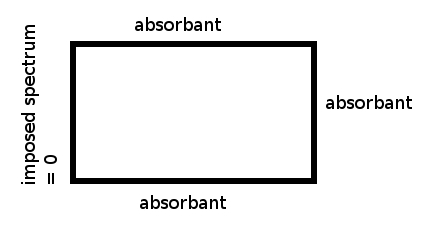
\includegraphics[width=0.85\textwidth]{boundarycond.jpg}
\caption{Boundary conditions}
\label{boundaryfet}
\end{figure}
\subsection{Numerical parameters}
\begin{itemize}
\item time step : 900~s
\item physical time reached : 48 h
\item caracterization of the computer : \subitem Core : Linux 2.6.32-5-amdb64 \subitem Processors : Intel(R)
xeon(R) CPU E5620 @ 2.4Ghz
\item CPU times : \\
\begin{tabular}{ccccc}
\toprule
\toprule
 & \textbf{tests 1/2/3/4} & \textbf{test 5/6} & \textbf{tests 6b} & \textbf{tests 7}\\
\midrule
CPU times & 3~min & 3h25 & 5h40 & 25 s \\
\bottomrule
\bottomrule
\end{tabular}
\end{itemize}

\section{Results - infinite depth }
\subsection{Wave growth depending on the fetch for different wind velocities.}
Figure \ref{hsfet} shows the significant wave heights and the peak periods of waves along the fetch (along the axis $ y = 250~m$ ) for the test 1 (the others are not shown because they give the same conclusions). These curves are obtained after 48 hour of wind action for a wind of 5 to 25 m/s. It is clearly seen that the wind has a considerable impact on these values and bigger waves are obtained with stronger wind. Also, stronger is the wind, longer is the fetch needed to reach the steady state. It can be noticed that the significant wave height does not grow linearly but following the squared wind velocity.
\begin{figure}[H]
  \centering
  	\includegraphics[width=0.5\textwidth]{Hm0_free_mesh.jpg}\includegraphics[width=0.5\textwidth]{Tp_free_mesh.jpg}
      \caption{Significant wave heights and peak periods for the first test, $U_{10} = 5 - 10 - 15 - 20 - 25 m/s$}
\label{hsfet}
\end{figure}
\subsection{Non-dimensionnal variances and peak frequencies.}
Here all the tests are compared, but only with a 20~m/s and 10~m/s winds. The values obtained with TOMAWAC V6P2 are compared with the empirical formulas : JONSWAP \cite{Hasselmann1973}, CERC (1977)\cite {CERC77}, Wilson \cite{Wilson1965}, Kahma \cite{Kahma1992}. The non-dimensional variables are :\\
\begin{itemize}
\item Non-dimensional Fetch : $x* = \frac{g x}{U_{10}^2}$
\item Non-dimensional variance : $m_{0}* = \frac{g^2 m_{0}}{U_{10}^4}$
\item Non-dimensional peak frequency : $f_{p}* = \frac{U_{10} f_{p}}{g}$
\end{itemize}
Where $U_{10}$ is the wind velocity at 10 meters from the sea.\\
\begin{figure}[H]
  \centering
  	\includegraphics[width=0.5\textwidth]{M0v10id.pdf}\includegraphics[width=0.5\textwidth]{M0v20id.pdf}\\
  	\includegraphics[width=0.5\textwidth]{fpv10id.pdf}\includegraphics[width=0.5\textwidth]{fpv20id.pdf}\\
      \caption{Comparison of normalized Variance M0* and normalized peak frequencies fp* for U10 = 10m/s (left) and 20m/s (right), m0* MP-A and fp* PM-A are , respectively, the variance and the peak frequency limits given by the revisited Pierson-Moskowitz formula from Alves \cite{Alves2003}}
\label{variancefet}
\end{figure}

Figure \ref{variancefet} shows the different results obtained. Generally, all tests give correct results, and stay close to the CERC, Wilson \& Goda and Kahma \& Calkoen curves.\\
The wind impact can be seen by two different behaviours. Indeed, for a 10~m/s wind, the results are really close to the empirical formula at small fetches. As the fetch grows, the differences between the models increrase, and the curves began to stray from the empirical formulas. In this case, the models of tests 1, 6 and 6b give the best results. At 20~m/s, a different behaviour is noticed: at small fetch the results are quite different from the empirical curves and it is only when the fetch grows that they match well with the empirical formula. In this case it is the model of test 5 which gives the best results. It can be concluded that there is a range where TOMAWAC results are really correct whatever the models used. For strong winds, an exact resolution of the quadruplet transfers, Snyder's wind generation model and Westhuysen white capping model (test 5) give better results at small fetch. \\
Thus, the analysis of Figure \ref{variancefet} shows a good matching between the  TOMAWAC wave simulations and the empirical formulas. A comparison was also done with the revisited Pierson-Moskowitz asymptotic limits from Alves and Banner \cite{Alves2003} for fully developed wind waves, the $U_{10}$-scaled asymptotes is added on Figure \ref{variancefet}. The formula gives:
\[\epsilon = (4.02 \pm 0.62)*10^{-3}\]
\[\nu = (1.23 \pm 0.08)* 10^{-1}\]
 It seems that the non-dimensional peak frequency $f_p*$ is a little bit over-estimated and the non-dimensional variance is a bit underestimated. Indeed, the empirical formula given by CERC (1984), which is used as a criterion for fully developed seas, to calculate the minimum fetch during the minimum duration (48h), is : $\frac{t_{min} g}{U_{10}} = 68.8 (\frac{X_{min} g}{U_{10}^2})^{0.67}$. Applying this formula we found that the fully developed seas are reached around $1 117~km$ for a 10 m/s wind and around $1 672 km$ for a 20 m/s wind. Thus, the fully developed sea may not be entirely reached at our last point ($X_{10} = 1000km$), which may explain the growth of the variance spectrum for some of the tests (see next subsection).

\subsection{Variance spectrum for a constant wind.}
In this subsection, we look at the development of the variance spectrum $E(f)$ along the fetch.
\[ E(f) = \int_{0}^{2\pi} F(f,\theta )d\theta
\]
The spectra are worked out for different points of fetch and for two wind speeds (10~m/s and 20~m/s):\\
\begin{center}
\begin{tabular}{c|c}
Points & fetch\\
\hline
Point 1 & 25 km \\
Point 2 & 50 km \\
Point 3 & 100 km \\
Point 4 & 150 km \\
Point 5 & 200 km\\
Point 6 & 300 km \\
Point 7 & 400 km \\
Point 8 & 800 km\\
Point 9 & 750 km\\
Point 10 & 1000 km\\
\end{tabular}\\
\end{center}
Dimensional variance spectrum (not shown here) gives correct results with a big growth of the peak value with the wind.\\
The non-dimensional frequency is defined by: $f* = \frac{U_{10}*f}{g}$.\\
and the variance spectra are normalised by the peak value of the Pierson-Moskowitz spectrum, which corresponds to the steady state:\\
$E_{PM}(f_{PM}) = \frac{\alpha g^2}{(2\pi)^4 f_{PM}^5} exp(-5/4)$ with $f_{PM}=\frac{0.13 g}{U_{10}}$ and the Philipp's constant $\alpha = 0.0081$\\
\begin{figure}[h!]
\begin{tabular}{cc}
\includegraphics[width=0.5\textwidth]{variance_ad_free_mesh_t1_v10.pdf} & \includegraphics[width=0.5\textwidth]{variance_ad_free_mesh_t1_fine_v20.pdf}\\
\includegraphics[width=0.5\textwidth]{variance_ad_free_mesh_t2_v10.pdf} & \includegraphics[width=0.5\textwidth]{variance_ad_free_mesh_t2_v20.pdf}\\
\includegraphics[width=0.5\textwidth]{variance_ad_free_mesh_t3_v10.pdf} & \includegraphics[width=0.5\textwidth]{variance_ad_free_mesh_t3_v20.pdf}\\
\includegraphics[width=0.5\textwidth]{variance_ad_free_mesh_t4_v10.pdf} & \includegraphics[width=0.5\textwidth]{variance_ad_free_mesh_t4_v20.pdf}\\
\end{tabular}
\caption{Comparaison of normalized spectrum variance for part one of the different tests and U10 = 10m/s (left) and 20m/s (right).}
\label{variancesfet1}
\end{figure} \begin{figure}[h!]
\begin{tabular}{cc}
\includegraphics[width=0.5\textwidth]{variance_ad_free_mesh_t5_v10.pdf} & \includegraphics[width=0.5\textwidth]{variance_ad_free_mesh_t5_v20.pdf}\\\\
\includegraphics[width=0.5\textwidth]{variance_ad_free_mesh_t6_v10.pdf} & \includegraphics[width=0.5\textwidth]{variance_ad_free_mesh_t6_fine_v20.pdf}\\
\includegraphics[width=0.5\textwidth]{variance_ad_free_mesh_t6b_v10.pdf} & \includegraphics[width=0.5\textwidth]{variance_ad_free_mesh_t6b_v20.pdf}\\
\end{tabular}
\caption{Comparaison of normalized spectrum variance for part2 of the different tests and U10 = 10m/s (left) and 20m/s (right).}
\label{variancesfet2}
\end{figure}
On Figure \ref{variancesfet1} and \ref{variancesfet2}, non-dimensional variance spectra can be observed. We can notice that as the fetch grows, the variance spectrum amplitude grows and the peak frequency declines. Moreover, the variance spectrum tends to the Pierson-Moskowitz spectrum for some cases. The exact quadruplet transfers calculation impact can be seen on the test 5, 6 and 6b, the shape of the curve changes, the spectrum is more peaked and the maximum value is higher, and it allows to observe a spectrum peak overstepping the state value predicted by Pierson-Moskowitz formula, it is an overshoot (test 6 for $U_{10} = 20m/s$ and test 6b).\\
For $U10 = 10m/s$, the last fetch points (points 7, 8, 9 and 10) get really close spectra. We can conclude that from a certain fetch, the fully developed sea state is reached. Althought, for the case $U10 = 20m/s$, the spectrum continues to grow and the overshoot's presence shows that this balance state is not yet reached. Thus, TOMAWAC gives good results which can be improved with the exact GQM quadruplet transfers model.

\subsection{Finite depth TOMAWAC results}
In this subsection, finite depths are considered : 180~m, 60~m, 30~m, 15~m and 5~m. In regards of Miche's criterion (1994), excepted for a 5 meters depth and $V = 20~m/s$, there is no bathymetric breaking dissipation. All the tests are done for the same generation (Snyder), white capping (Westhuysen) and quadruplet transfer (DIA) models. Figure \ref{variancem0} shows the evolution of the non-dimensional variance along the fetch for the different tests. In order to compare with the CERC (1984) parametrization, non-dimensional variables are defined as:\\
\begin{itemize}
\item CERC parametrization (1984) :
\subitem $X* = \frac{g*X}{U_a}$
\subitem $U_a = 0.71*U_{10}^{1.23}$
\subitem $m0* = \frac{g^2*m0}{U_a^4}$
\end{itemize}
It can be noticed that the non-dimensional variance decreases with depth. Indeed, bottom friction effects are more important at small depths. On the contrary, the peak frequency grows when the depth increases because the friction has more impact on small frequency waves, which leads to a growth of the peak frequency.\\
On Figure 6, we can see that for a 20 m/s wind, TOMAWAC curves are really matching with the CERC (1984) forecasting, particularly for $d = 15 - 30 - 60~m$. Indeed, it is adviced in CERC publication to use their model for a depth between 15 and 90 meters. But the results are still good for $d = 180~m$ and $d = 5~m$.\\
For a 10m/s wind, except for $d = 5~m $ and $d = 15 m$, the results are less close to the CERC curves. At small fetches, TOMAWAC results are overvalued, and at large fetches, they are undervalued. In CERC publication (1984), it is adviced to use an infinite model for depth over 90m. So the CERC infinite depth model (1977) is added to the graphs and we can see that the results are closer to it for a 10 m/s wind and $d \geq 30m$.For a 20 m/s wind,at $d = 180m$ and at large fetches, TOMAWAC results tends to the infinite depth limit.
\begin{figure}
\centering
\includegraphics[width=0.85\textwidth]{m0_test7v10.pdf}\\
\includegraphics[width=0.85\textwidth]{m0_test7v20.pdf}\\
\caption{Comparaison of normalized Variance M0* for U10 = 10m/s (high) and 20m/s (bottom) for different depths : 5, 15, 30, 60, 180 m}
\label{variancem0}
\end{figure}
Generally, TOMAWAC gives correct results if you adapt the good model at the application.
\section{Conclusion}
\subsection{Infinite Depth}
This benchmark allows to verify that TOMAWAC results for simultaneous processing of different source terms are correct. A comparison with empirical formulas validates this simulation with generally matching results. The use of the exact GQM quadruplet transfers model allows the visualization of overshoots, but,CPU time are increased, so it is not advisable to use this model for big industrial cases.
\begin{figure}[h!]
  \centering
  \includegraphicsmaybe{[width=0.85\textwidth]}{../img/resultsinfinite.png}
  \caption{wave heigth for infinite depth}
\label{resultinfinite}
\end{figure}

\subsection{Finite depth}
Even if a 1000 km fetch with only 5 m depth is hard to study in reality, TOMAWAC results get close to the empirical formula. Bottom friction effect seems to be well represented.
\begin{figure}[h!]
  \centering
  \includegraphicsmaybe{[width=0.85\textwidth]}{../img/resultsfinite.png}
  \caption{wave heigth for finite depth}
\label{finite}
\end{figure}


\subsection{Some Tests}
We present Figures \ref{test4} \ref{test6} and \ref{test6b} some results of other tests. The references for the comparison are made with the version 7.2 of \tomawac.   
\begin{figure}[h!]
  \centering
  \includegraphicsmaybe{[width=0.85\textwidth]}{../img/resultstest4.png}
  \caption{wave heigth for test4}
\label{test4}
\end{figure}
\begin{figure}[h!]
  \centering
  \includegraphicsmaybe{[width=0.85\textwidth]}{../img/resultstest6.png}
  \caption{wave heigth for test6}
\label{test6}
\end{figure}
\begin{figure}[h!]
  \centering
  \includegraphicsmaybe{[width=0.85\textwidth]}{../img/resultstest6b.png}
  \caption{wave heigth for test6b}
\label{test6b}
\end{figure}
